\documentclass[english]{exercisesheet}

\usepackage{bm}
\usepackage{mymath}
\usepackage{graphicx}

\author{Daniel Strenger, Lorenzo Minneci}
\immatriculationnumber{01531211, 11939539}
\semester{SS 2020}
\subject{Machine Learning}
\sheetnumber{3}

\begin{document}
 \makedocumentheader
  \begin{nexercise}{Datasets}
      \begin{solution} 1.
        \begin{figure}
        \centering
        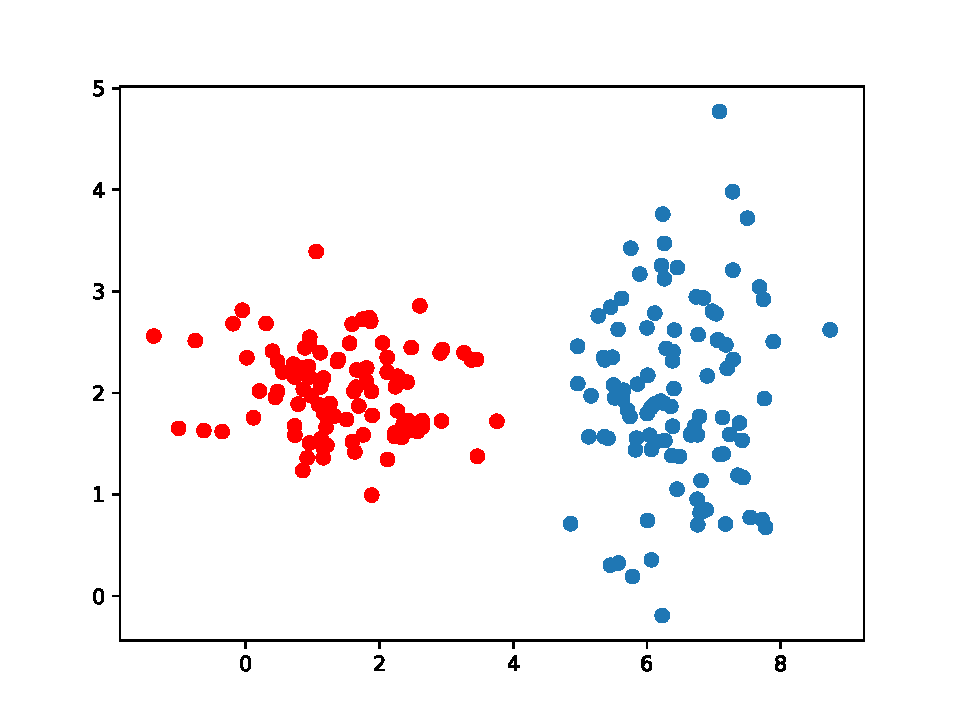
\includegraphics[width=10cm]{simple.pdf}
        \caption{$\sigma_{r}^{2} = 6$}
        \end{figure}
        \begin{figure}
        \centering
        \cleardoublepage
        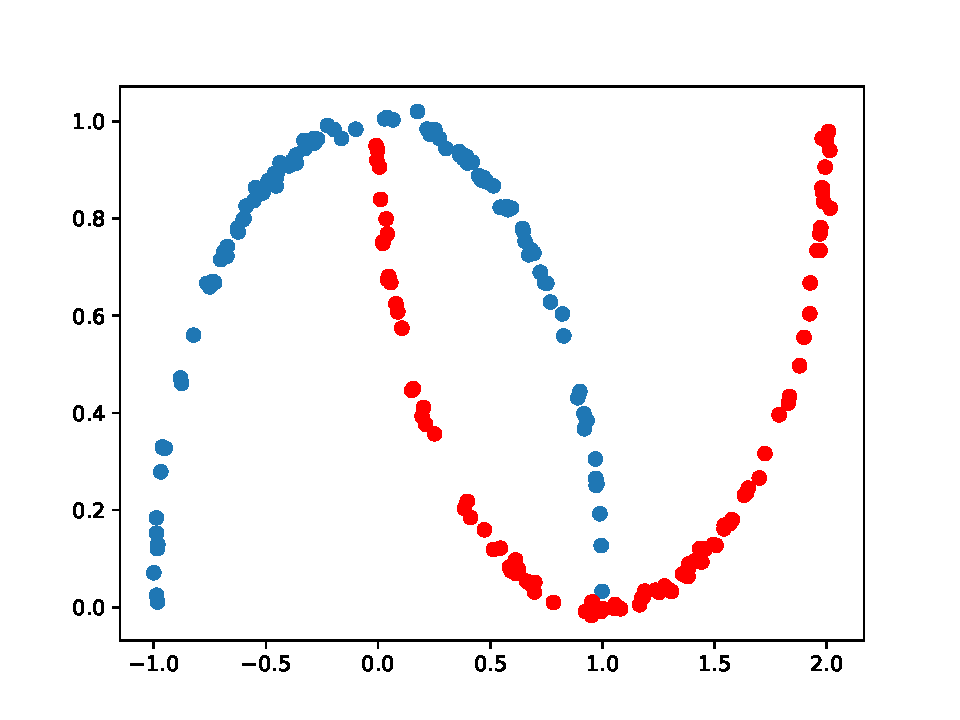
\includegraphics[width=10cm]{moon.pdf}
        \caption{$\sigma_{r}^{2} = 0.1$}
        \end{figure}
    \end{solution}
  
 \end{nexercise}
 
 \cleardoublepage
 \begin{nexercise}{Support Vector Machine - Primal Problem}
 \begin{solution} 2.
        \begin{figure}
        \centering
        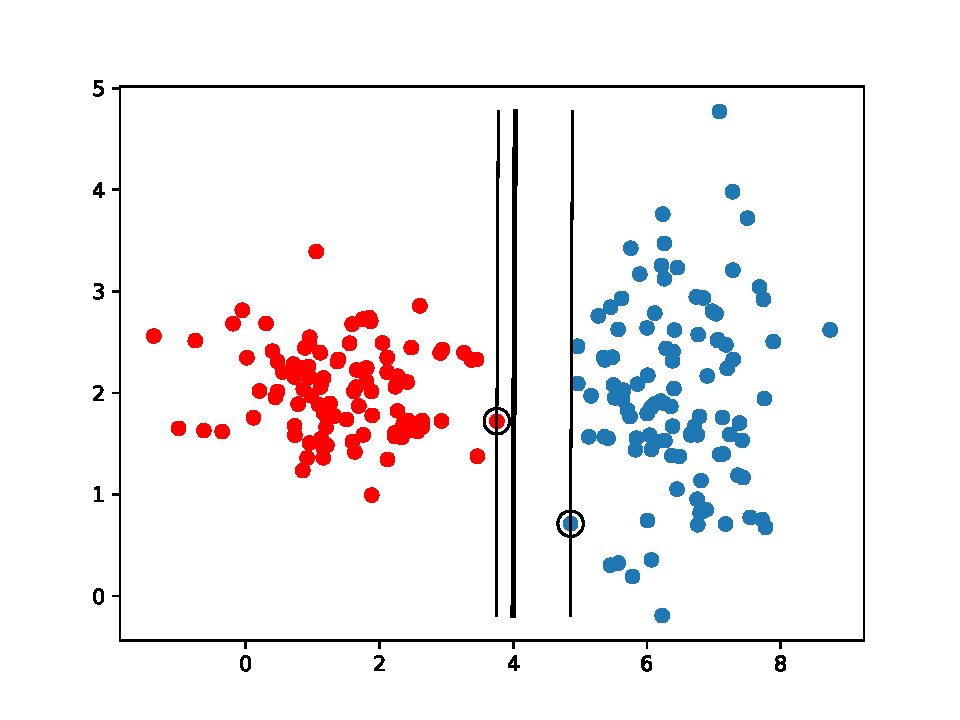
\includegraphics[width=10cm]{simple-line.pdf}
        \caption{First dataset, SVM}
        \end{figure}
        \begin{figure}
        \centering
        \cleardoublepage
        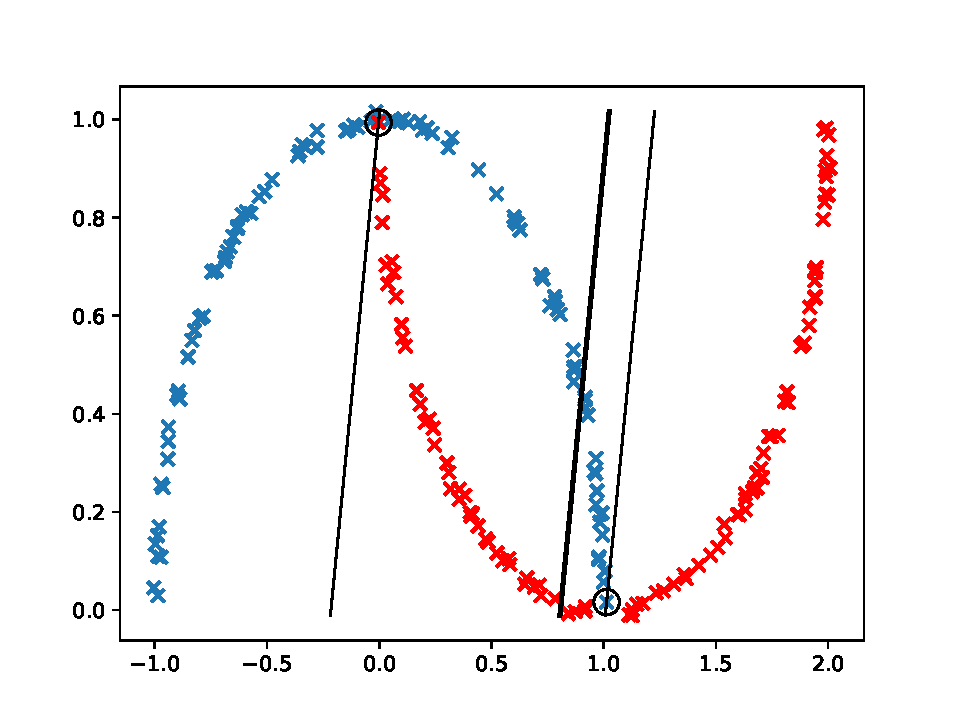
\includegraphics[width=10cm]{moon-line.pdf}
        \caption{Halfmoon dataset, SVM}
        \end{figure}
    \end{solution}
 
 We can notice that in the first example the SVM machine is clearly able to divide the two data sets, even if one of the two dimensions (the Y axis) is not significant for the classification problem. Ideally we could have just used the feature in the x axis for the problem.
 
 In the second example we notice that the SVM is not able to distinguish between the two data sets. This happen due to the linearity of the function used to divide the classes.
 
 \end{nexercise}
 
\end{document}
